\documentclass[a4paper, 9pt, twocolumn]{extarticle}
\usepackage{amsmath,graphicx,amssymb,cite}
\usepackage[utf8]{inputenc}
\usepackage[english]{babel}

\usepackage{url}


\addtolength{\textwidth}{2.1cm}
\addtolength{\topmargin}{-2.4cm}
\addtolength{\oddsidemargin}{-1.1 cm}
\addtolength{\textheight}{4.5cm}
\setlength{\columnsep}{0.7cm}

% User defined macros
\def\x{{\mathbf x}}
\def\L{{\cal L}}
\def\SM{{\mathcal S}}
\def\SMO{{\mathcal S^{\mathrm{chroma}}}}
\def\SMS{{\mathcal S^{\mathrm{enh}}}}
\def\SMP{{\mathcal S^{\mathrm{path}}}}
\def\SMPI{{\mathcal S^{\mathrm{struct}}}}
%\def\SMPC{{\mathcal S^{\mathrm{pc}}}}
\def\SMPC{{\mathcal S^{\mathrm{pb}}}}

\pagestyle{empty}

\begin{document}

\date{\normalsize 01.01.2024}

\title{\vspace{-8mm}\textbf{\Large
Title of the Summary\footnote{This is the summary for the reading assignment,
which is part of the exercise of the lecture \emph{Music Processing Analysis}, Winter Term 2023/24,
Friedrich-Alexander Universit\"at Erlangen-N\"urnberg.
Instructor: Prof.\ Dr.\ Meinard M\"uller,
Tutor: Simon Schw\"ar.
}}}

% Hier die Namen und Daten der beteiligten Autoren eintragen
\author{
{
\begin{minipage}{\textwidth}
\center
Max Mustermann\\
\small
Friedrich-Alexander Universit\"at Erlangen-N\"urnberg
\protect\\{} %
\url{max.mustermann@FAU.de}
\end{minipage}
}
}

\maketitle
\thispagestyle{empty}

%%%%%%%%%%%%%%%%%%%%%%%%%%%%%%%%%%%%%%%%%%%%%%%%%%%%%%%%%%%%%%%%%%%%%%%%%%%%%%
\section{Introduction}
\label{section:introduction}
%%%%%%%%%%%%%%%%%%%%%%%%%%%%%%%%%%%%%%%%%%%%%%%%%%%%%%%%%%%%%%%%%%%%%%%%%%%%%%

This chapter focuses on the process of music synchronization, which
involves aligning different musical representations, such as audio
recordings and sheet music. The core concept is to extract meaningful
features from these representations and then employ a technique called
Dynamic Time Warping (DTW) to find the optimal temporal correspondence
between them.
\section{Audio Features}
The chapter emphasizes the importance of \textbf{chroma features} in music
synchronization. Chroma features essentially capture the distribution of
energy across the 12 pitch classes (C, C\#, D, ..., B) while
disregarding octave information. This characteristic makes them robust
to variations in timbre and dynamics, allowing for effective comparison
of different musical interpretations.
\subsection{Log-Frequency Spectrogram}
The process of extracting chroma features starts with a
\textbf{log-frequency spectrogram}. The \emph{Log-Frequency Spectrogram}
elucidates the transformation of an audio recording into a
representation that reveals the energy distribution across different
pitches. This is a crucial step in music synchronization as it makes
music data comparable and algorithmically accessible.

The process leverages the \textbf{logarithmic perception of frequency in
human hearing} and aims to create a time-frequency representation where
the frequency axis is logarithmic and labeled by the pitches of the
equal-tempered scale.

Here\textquotesingle s a breakdown of the process:

\begin{enumerate}
\def\labelenumi{\arabic{enumi}.}
\item
  \textbf{Starting with a spectrogram:} The spectrogram, obtained using
  the Short-Time Fourier Transform (STFT), provides a visual
  representation of the frequency content of an audio signal over time.
\item
  \textbf{Mapping to the Equal-Tempered Scale:} Each spectral
  coefficient in the spectrogram is assigned to a pitch in the
  equal-tempered scale. This is done by finding the pitch whose center
  frequency is closest to the frequency of the spectral coefficient.
\item
  \textbf{Creating the Log-Frequency Spectrogram:} A log-frequency
  spectrogram is then generated by grouping the spectral coefficients
  according to their assigned pitches. For each pitch, the squared
  magnitudes of the corresponding spectral coefficients are summed up.
  This results in a representation where the frequency axis is now
  logarithmic and labeled by MIDI pitches.
\end{enumerate}

However, this process encounters challenges, particularly in
representing low pitches:

\begin{itemize}
    \item
      \textbf{Limited Frequency Resolution:} The STFT\textquotesingle s
      linear frequency sampling can be insufficient to accurately represent
      the lower pitches due to their narrower bandwidths in the logarithmic
      scale. This can lead to a poor representation of low-frequency
      content.
    \item
      \textbf{Trade-off Between Time and Frequency Resolution:} Increasing
      the window length in the STFT can improve frequency resolution but
      leads to a decrease in temporal resolution, potentially losing crucial
      information about note onsets.
    \end{itemize}
    
    A solution to these challenges is a \textbf{multiresolution approach}.
    This involves using multiple spectrograms computed with different
    sampling rates and window sizes. A higher sampling rate and shorter
    window are used for high pitches to prioritize temporal resolution,
    while a lower sampling rate and longer window are used for low pitches
    to prioritize frequency resolution.
    
    From this log-frequency spectrogram, the \textbf{chromagram} is derived
    by summing up all pitch coefficients that belong to the same chroma. The
    \emph{chroma features} represent the harmonic content of music. This
    representation is fundamental to music synchronization as it captures
    the essential harmonic information while remaining robust to variations
    in timbre and instrumentation.
    \subsection{Chroma features}
    Chroma features are derived from the log-frequency spectrogram
    and essentially aggregate all spectral information related to a
    particular pitch class into a single coefficient.
    
    The process involves the \textbf{Pitch Class Aggregation,} Which For
    each of the 12 chroma values (C, C\#, D, ..., B), all the pitch
    coefficients in the log-frequency spectrogram belonging to the same
    chroma are summed up. This means that all notes that are an octave apart
    (like C1, C2, C3) contribute to the same chroma band.
    
    This results in a \textbf{chromagram}, a time-chroma representation
    where each time frame is characterized by a 12-dimensional vector
    representing the energy distribution across the 12 chroma values.
    
    The highlights the following \textbf{advantages of using chroma
    features}:
    
    \begin{itemize}
    \item
      \textbf{Robustness to Timbre Variations:} By aggregating the energy of
      octaves, chroma features become largely invariant to the specific
      timbre of the instrument or sound source. This allows us to compare
      different performances or interpretations of the same musical piece
      even if they use different instruments.
    \item
      \textbf{Compact Representation of Harmony:} Chroma features
      effectively condense the information from the 128 pitch bands of the
      log-frequency spectrogram into 12 chroma bands, providing a more
      concise representation of the harmonic content.
    \end{itemize}
    
    However, this reduction in dimensionality also results in some loss of
    information. For instance, notes with the same chroma but in different
    octaves become indistinguishable in the chromagram.
    
    Some technics which can help us to not lose information:
    
\begin{itemize}
    \item
      \textbf{Logarithmic Compression:} Applying logarithmic compression to
      the chromagram reduces the dynamic range of the features, emphasizing
      weaker but potentially significant harmonic components that might
      otherwise be overshadowed by stronger components.
    \item
      \textbf{Normalization:} Normalizing the chroma vectors ensures that
      they are invariant to changes in dynamics, making comparisons between
      different performances or sections of music more meaningful.
    \end{itemize}
    
    Furthermore, the \textbf{cyclic nature of chroma features} is explaining
    how a cyclic shift of the chroma vector can simulate transpositions of
    music. It concludes by emphasizing that the choice of specific chroma
    feature variants and processing techniques depends heavily on the
    intended application.

    \section{Dynamic Time Warping (DTW)}
   Dynamic Time Warping (DTW) is then introduced as a technique
    for aligning two sequences of chroma features.
    \subsection{ Basic Approach}
    DTW aims to find an optimal alignment that minimizes the total cost of matching
    corresponding elements in the sequences, effectively compensating for
    differences in tempo between different musical interpretations.
    
    A \textbf{warping path} represents the alignment between the two
    sequences, defined as a sequence of index pairs that satisfy specific
    conditions:
    
    \begin{itemize}
    \item
      \textbf{Boundary condition}: The path starts at the beginning of both
      sequences and ends at the end of both sequences.
    \item
      \textbf{Monotonicity condition}: The path progresses monotonically
      through both sequences, reflecting faithful timing.
    \item
      \textbf{Step size condition}: The path only allows for specific
      movements between cells of the cost matrix, ensuring a continuous
      alignment.
    \end{itemize}
    
    The \textbf{total cost} of a warping path is calculated by summing up
    the local cost of aligning each pair of elements connected by the path.
    An \textbf{optimal warping path} is the one with the minimal total cost
    among all possible paths, and the \textbf{DTW distance} between two
    sequences is defined as the total cost of this optimal path.
    
    Moreover, A \textbf{dynamic programming algorithm} for efficiently
    computing the DTW distance and the corresponding optimal warping path.
    The algorithm operates by recursively building an accumulated cost
    matrix, where each entry represents the minimum cost of aligning
    prefixes of the two input sequences.
    \subsection{DTW variants}
    Several DTW variants are presented, each offering specific
    controls and optimizations for the alignment process:
    
    \begin{itemize}
    \item
      \textbf{Modified Step Size Condition}: By adjusting the allowed steps
      in the warping path, it is possible to constrain the local slope of
      the alignment, preventing overly stretched or compressed sections.
    \item
      \textbf{Local Weights}: Different weights can be assigned to vertical,
      horizontal, and diagonal steps in the warping path, allowing for
      preferences in the alignment direction.
    \item
      \textbf{Global Constraints}: By restricting the admissible warping
      paths to specific regions within the cost matrix, such as the
      Sakoe-Chiba band or the Itakura parallelogram, computational
      efficiency can be improved and pathological alignments avoided.
    \item
      \textbf{Multiscale DTW}: This approach uses a hierarchical strategy,
      starting with a coarse alignment at a low resolution and then refining
      it at progressively higher resolutions, allowing for more efficient
      and robust alignment of long sequences.
    \end{itemize}
    \section{Applications}
    A few applications of music synchronization:
    
    \begin{itemize}
    \item
      \textbf{Multimodal Music Navigation}: Synchronization results can be
      used to create user interfaces that allow users to browse and explore
      music in a multimodal way. An example is the \textbf{Interpretation
      Switcher}, which enables seamless switching between different
      recordings of the same musical work.
    \item
      \textbf{Score Viewer Interface}: This interface provides a
      synchronized view of sheet music and an audio recording, highlighting
      the corresponding musical measures during playback.
    \item
      \textbf{Tempo Curves}: By aligning a performance to a reference score,
      it is possible to extract tempo curves that represent the relative
      tempo changes in the performance compared to the reference.
    \end{itemize}
    \section{In The End}
    The chapter provides a comprehensive overview of the key
    concepts, techniques, and applications of music synchronization,
    highlighting the role of chroma features and Dynamic Time Warping in
    aligning different musical representations. It also emphasizes the
    importance of understanding the various DTW variants and their impact on
    the alignment process, and showcases the potential of music
    synchronization for enhancing the user experience and facilitating music
    analysis.
    \section{Feedback}
    \begin{itemize}
      \item This report helped me better understand the DTW variants, and I really liked the technique related to Multiscale DTW.
      \item I did not mention the online approach of DTW because did not understand it.
    \end{itemize}
% %%%%%%%%%%%%%%%%%%%%%%%%%%%%%%%%%%%%%%%%%%%%%%%%%%%%%%%%%%%%%%%%%%%%%%%%%%%%%%
% \section{Main Section}
% \label{section:main}
% %%%%%%%%%%%%%%%%%%%%%%%%%%%%%%%%%%%%%%%%%%%%%%%%%%%%%%%%%%%%%%%%%%%%%%%%%%%%%%
% This chapter focuses on the process of music synchronization, which involves aligning different musical representations, such as audio recordings and sheet music. The core concept is to extract meaningful features from these representations and then employ a technique called Dynamic Time Warping (DTW) to find the optimal temporal correspondence between them.
% The text emphasizes the importance of chroma features in music synchronization. Chroma features essentially capture the distribution of energy across the 12 pitch classes (C, C\verb|#|, D, ..., B) while disregarding octave information. This characteristic makes them robust to variations in timbre and dynamics, allowing for effective comparison of different musical interpretations.
% The process of extracting chroma features starts with a log-frequency spectrogram. This spectrogram is generated by transforming an audio recording using the Short-Time Fourier Transform (STFT), which represents the audio signal's frequency content over time. The frequency axis of this spectrogram is then converted from Hertz to a logarithmic scale based on the pitches of the equal-tempered scale, resulting in the log-frequency spectrogram.
% From this log-frequency spectrogram, the chromagram is derived by summing up all pitch coefficients that belong to the same chroma. The resulting chroma features are robust to variations in timbre and instrumentation.
% The text further discusses various preprocessing techniques that can enhance the quality and effectiveness of chroma features, including:
% •	Logarithmic Compression: This step helps to balance out the large dynamic range of chroma features, enhancing the small but relevant values that may be obscured by larger values.
% •	Normalization: This process ensures that the chroma vectors are invariant to changes in dynamics, making them more comparable.
% Dynamic Time Warping (DTW) is then introduced as a technique for aligning two sequences of chroma features. DTW aims to find an optimal alignment that minimizes the total cost of matching corresponding elements in the sequences, effectively compensating for differences in tempo between different musical interpretations.
% A warping path represents the alignment between the two sequences, defined as a sequence of index pairs that satisfy specific conditions:
% •	Boundary condition: The path starts at the beginning of both sequences and ends at the end of both sequences.
% •	Monotonicity condition: The path progresses monotonically through both sequences, reflecting faithful timing.
% •	Step size condition: The path only allows for specific movements between cells of the cost matrix, ensuring a continuous alignment.
% The total cost of a warping path is calculated by summing up the local cost of aligning each pair of elements connected by the path. An optimal warping path is the one with the minimal total cost among all possible paths, and the DTW distance between two sequences is defined as the total cost of this optimal path.
% The text then details a dynamic programming algorithm for efficiently computing the DTW distance and the corresponding optimal warping path. The algorithm operates by recursively building an accumulated cost matrix, where each entry represents the minimum cost of aligning prefixes of the two input sequences.
% Several DTW variants are presented, each offering specific controls and optimizations for the alignment process:
% •	Modified Step Size Condition: By adjusting the allowed steps in the warping path, it is possible to constrain the local slope of the alignment, preventing overly stretched or compressed sections.
% •	Local Weights: Different weights can be assigned to vertical, horizontal, and diagonal steps in the warping path, allowing for preferences in the alignment direction.
% •	Global Constraints: By restricting the admissible warping paths to specific regions within the cost matrix, such as the Sakoe-Chiba band or the Itakura parallelogram, computational efficiency can be improved and pathological alignments avoided.
% •	Multiscale DTW: This approach uses a hierarchical strategy, starting with a coarse alignment at a low resolution and then refining it at progressively higher resolutions, allowing for more efficient and robust alignment of long sequences.
% The text concludes by discussing various applications of music synchronization techniques:
% •	Multimodal Music Navigation: Synchronization results can be used to create user interfaces that allow users to browse and explore music in a multimodal way. An example is the Interpretation Switcher, which enables seamless switching between different recordings of the same musical work.
% •	Score Viewer Interface: This interface provides a synchronized view of sheet music and an audio recording, highlighting the corresponding musical measures during playback.
% •	Tempo Curves: By aligning a performance to a reference score, it is possible to extract tempo curves that represent the relative tempo changes in the performance compared to the reference.
% In summary, the text provides a comprehensive overview of the key concepts, techniques, and applications of music synchronization, highlighting the role of chroma features and Dynamic Time Warping in aligning different musical representations. It also emphasizes the importance of understanding the various DTW variants and their impact on the alignment process, and showcases the potential of music synchronization for enhancing the user experience and facilitating music analysis.

% %%%%%%%%%%%%%%%%%%%%%%%%%%%%%%%%%%%%%%%%%%%%%%%%%%%%%%%%%%%%%%%%%%%%%%%%%%%%%%
% % Here you find some additional LaTex code fragments for including figures and
% % references which you may find helpful.
% %%%%%%%%%%%%%%%%%%%%%%%%%%%%%%%%%%%%%%%%%%%%%%%%%%%%%%%%%%%%%%%%%%%%%%%%%%%%%%

% Example for a citation:~\cite{Mueller21_FMP_SPRINGER}.

% Example for figure: Figure~\ref{figure:example}.

% \newpage

% %%%%%%%%%%%%%%%%%%%%%%%%%%%%%%%%%%%%%%%%%%%%%%%%%%%%%%%%%%%%%%%%%%%%%%%%%%%%%%
% \section{Feedback}
% \label{section:feedback}
% %%%%%%%%%%%%%%%%%%%%%%%%%%%%%%%%%%%%%%%%%%%%%%%%%%%%%%%%%%%%%%%%%%%%%%%%%%%%%%


% %-----------------------
% \begin{figure}[t]
%     \centering
%     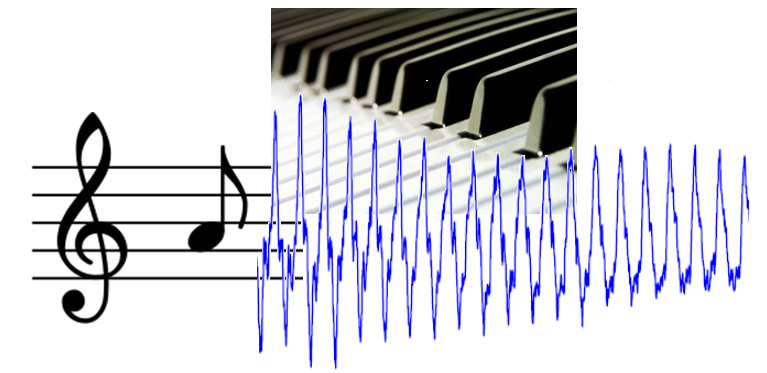
\includegraphics[width=5cm]{figure_example.png}
%     \caption{Example for a figure.}
%     \label{figure:example}
% \end{figure}
% %-----------------------


% Feedback may also be given in form of bullet points
% \begin{itemize}
%     \item This was good....
%     \item I did not like...
% \end{itemize}



%%%%%%%%%%%%%%%%%%%%%%%%%%%%%%%%%%%%%%%%%%%%%%%%%%%%%%%%%%%%%%%%%%%%%%%%%%%%%%%%%%%%%%%%%%%%%%%%%%
\bibliographystyle{abbrv}
\small
\bibliography{references}
%%%%%%%%%%%%%%%%%%%%%%%%%%%%%%%%%%%%%%%%%%%%%%%%%%%%%%%%%%%%%%%%%%%%%%%%%%%%%%%%%%%%%%%%%%%%%%%%%%



\end{document}
